\documentclass[a4paper, 12pt]{article}

%%% Работа с русским языком
\usepackage{cmap}					% поиск в PDF
\usepackage{mathtext} 				% русские буквы в формулах
\usepackage[T2A]{fontenc}			% кодировка
\usepackage[utf8]{inputenc}			% кодировка исходного текста
\usepackage[russian]{babel}	% локализация и переносы

%%% Дополнительная работа с математикой
\usepackage{amsmath,amsfonts,amssymb,amsthm,mathtools} % AMS
\usepackage{icomma} % "Умная" запятая: $0,2$ --- число, $0, 2$ --- перечисление

%% Номера формул
%\mathtoolsset{showonlyrefs=true} % Показывать номера только у тех формул, на которые есть \eqref{} в тексте.

%% Шрифты
\usepackage{euscript}	 % Шрифт Евклид
\usepackage{mathrsfs} % Красивый матшрифт

%% Поля
\usepackage[left=2cm,right=2cm,top=2cm,bottom=2cm,bindingoffset=0cm]{geometry}

%% Русские списки
\usepackage{enumitem}
\makeatletter
\AddEnumerateCounter{\asbuk}{\russian@alph}{щ}
\makeatother

%%% Работа с картинками
\usepackage{graphicx}  % Для вставки рисунков
\graphicspath{{images/}{images2/}}  % папки с картинками
\setlength\fboxsep{3pt} % Отступ рамки \fbox{} от рисунка
\setlength\fboxrule{1pt} % Толщина линий рамки \fbox{}
\usepackage{wrapfig} % Обтекание рисунков и таблиц текстом

%%% Работа с таблицами
\usepackage{array,tabularx,tabulary,booktabs} % Дополнительная работа с таблицами
\usepackage{longtable}  % Длинные таблицы
\usepackage{multirow} % Слияние строк в таблице

%% Красная строка
\setlength{\parindent}{2em}

%% Интервалы
\linespread{1}
\usepackage{multirow}

%% TikZ
\usepackage{tikz}
\usetikzlibrary{graphs,graphs.standard}

%% Верхний колонтитул
\usepackage{fancyhdr}
\pagestyle{fancy}

%% Перенос знаков в формулах (по Львовскому)
\newcommand*{\hm}[1]{#1\nobreak\discretionary{}
	{\hbox{$\mathsurround=0pt #1$}}{}}

%% Мои дополнения
\usepackage{float} %Добавляет возможность работы с командой [H] которая улучшает расположение на странице
\usepackage{gensymb} %Красивые градусы
\usepackage{graphicx}               % Импорт изображений
\usepackage{caption} % Пакет для подписей к рисункам, в частности, для работы caption*

% подключаем hyperref (для ссылок внутри  pdf)
\usepackage[unicode, pdftex]{hyperref}

%%% Теоремы
\theoremstyle{plain}                    % Это стиль по умолчанию, его можно не переопределять.
\renewcommand\qedsymbol{$\blacksquare$} % переопределение символа завершения доказательства

\newtheorem{theorem}{Теорема}[section] % Теорема (счетчик по секиям)
\newtheorem{proposition}{Утверждение}[section] % Утверждение (счетчик по секиям)
\newtheorem{definition}{Определение}[section] % Определение (счетчик по секиям)
\newtheorem{corollary}{Следствие}[theorem] % Следстиве (счетчик по теоремам)
\newtheorem{problem}{Задача}[section] % Задача (счетчик по секиям)
\newtheorem*{remark}{Примечание} % Примечание (можно переопределить, как Замечание)
\newtheorem{lemma}{Лемма}[section] % Лемма (счетчик по секиям)

\begin{document}
\newcommand{\HRule}{\rule{\linewidth}{0.7mm}} % Defines a new command for the horizontal lines, change thickness here
	
	\begin{center}
		\large\textbf{Московский Физико-Технический Институт}\\ % Name of your university/college
		\large\textbf{(государственный университет)}
	
		\vfill
		
		\Large Лабораторная работа по курсу общей физики № *labnum*\\[0.5cm] % Preambule of your document title
		
		
		\HRule
		\\[0.4cm]
		{ \huge \bfseries *name of your labwork*}% Title of your document
		\\[0.4cm] 
		\HRule
		\\[0.5cm]
		
		\ \\
	\textbf{\large Автор:} \\	
	\large *your name* *groupname*\\ % Your name and something more, your group num for example
		\vfill
		\hspace*{-0.8 cm}
\includegraphics[width=100 pt]{frkt_logo}\\ % logo of your  company/university/college
		\large Долгопрудный, 2021 % location and year
	\end{center}

\newpage
\setcounter{page}{2}
\fancyfoot[c]{\thepage}
\fancyhead[L] {Работа № *labnum*} % some information in page header
\fancyhead[R]{}

\textbf{Цель работы}: исследовать интерференцию рассеянного света, прошедшего кристалл; наблюдать изменение характера поляризации света при наложении на кристалл электрического поля.

\textbf{В работе используются}: гелий-неоновый лазер, поляризатор, кристалл ниобата лития, матовая пластина, экран, источник высоковольтного переменного и постоянного напряжения, фотодиод, осцилограф, линейка.

\section*{Теория}
Эффект Поккельса -- изменение показателя преломления света в кристалле под действием электрического поля.\\
Рассмотрим кристалл ниобата лития $\text{LiNbO}_3$ с цетрольноосевой симметрией вдоль оси $Z$. Для световой волны с $\mathbf{E}$ перпендикулярно $Z$ показатель преломления будет $n_o$, а для волны с $\mathbf{E}$ вдоль $Z$ -- $n_e$. В случае, когда луч света идёт под углом $\theta$ к оси, есть два значение показателя преломления $n_1$ и $n_2$: $n_1 = n_o$ для волны с $\mathbf{E}$ перпендикулярным плоскости $(\mathbf{k},\mathbf{Z})$ (обыкновенная волна) и $n_2$ для волны с $\mathbf{E}$ в этой плоскости (необыкновенная волна). В последнем случае

\begin{equation}
\dfrac{1}{n_2^2}=\dfrac{\cos^2 \theta}{n_0^2}+\dfrac{\sin^2 \theta}{n_e^2}.
\end{equation}

\begin{figure}[h!]
	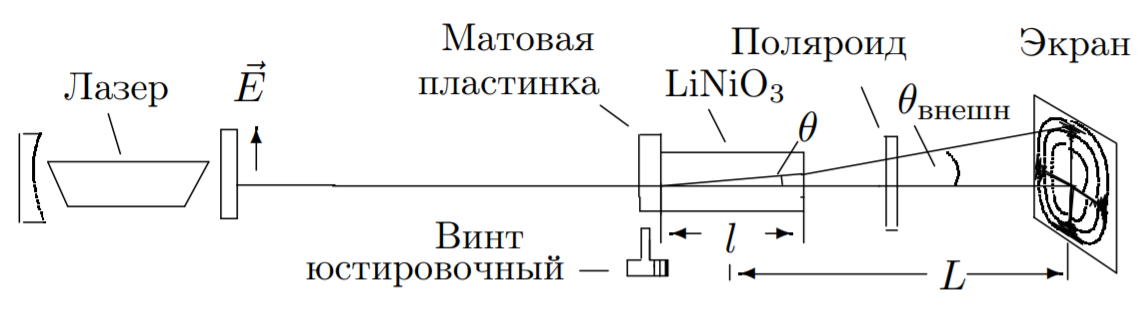
\includegraphics[scale=0.5]{1.png}
	\centering
	\caption{Схема для наблюдения интерфереционной картины}
	\label{fig:1}
\end{figure}

Если перед кристаллом, помещённым между поляроидами, расположить линзу или матовую пластинку, то на экране за поляроидом мы увидим тёмные концентрические окружности -- рещультат интерфернции обыкновенной и необыкновенной волн. При повороте выходного поляроида на $90^\circ$ картина меняется с позитива на негатив (на месте светлых пятен тёмные и наоборот). В случаи, когда разрешённое направление анализатора перпендикулярно поляризации лазерного излучения, радиус тёмного кольца с номером $m$ равен

\begin{equation} \label{eq:r(m)}
r_m^2 = \dfrac{\lambda}{l} \dfrac{(n_oL)^2}{n_0 - n_e}m,
\end{equation}

где $L$ -- расстояние от центра кристалла до экрана, $l$ -- длина кристалла.\\
Теперь поместим кристалл в постоянное электрическое поле $E_{\text{эл}}$, направленное вдоль оси $X$, перпендикулярной $Z$. Показатель преломления для луча, распространяющего вдоль $Z$, всегда $n_o$. В плоскости $(X,Y)$ возникают два главных направления под углами $45^\circ$ к $X$ и $Y$ с показателями преломления $n_0 - \Delta n$ и $n_o + \Delta n$ (быстрая и медленная ось), причём $\Delta n = A E_{\text{эл}}$. Для поляризованного вертикально света и анализатора, пропускающего горизонтальную поляризацию, на выходе интенсивность на выходе будет иметь вид

\begin{equation}
I_{\text{вых}} = I_0 \sin^2 \left(\dfrac{\pi}{2} \dfrac{U}{U_{\lambda/2}} \right),
\end{equation}
где $U_{\lambda/2} = \frac{\lambda}{4A}\frac{d}{l}$ -- \textit{полуволновое напряжение}, $d$ -- поперечный размер кристалла.  При напряжении $U = E_{\text{эл}}d$ равном полуволновому сдвиг фаз между двумя волнами равен $\pi$, а интенсивность света на выходе максимальна. 


\begin{figure}{r}
	\centering
	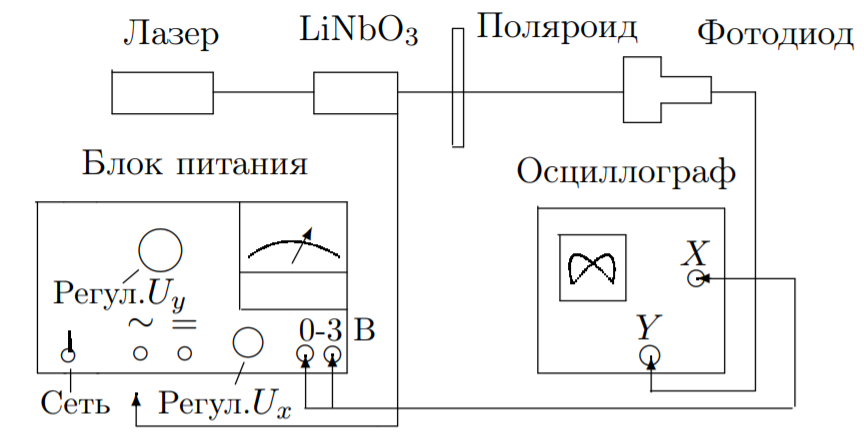
\includegraphics[width = 0.45\textwidth]{2.png}
	\caption{Схема установки.}
	\label{fig:scheme}
\end{figure}

На рис \ref{fig:scheme} представлена схема всей установки (оптическая часть изорбажена на рис \ref{fig:1}). Свет лазера, проходя через сквозь пластину, рассеивается и падает на двоякопреломляющий кристалл. На экране за поляроидом видна интерференционная картина. Убрав рассеивающую пластину и подавая на кристалл постоянное напряжение, можно величиной напряжения влиять на поляризацию луча, вышедшего из кристалла. Заменив экран фотодиодом и подав на кристалл переменное напряжение, можно исследовать поляризацию с помощью осциллографа.

\section*{Ход работы}

Запишем параметры установки

\begin{center}
	$\lambda = 0.63$ мкм \\
	$n_0 = 2.29$ \\
	$\varphi = 88^o$ -- угол поворота анализатора \\
	$L = 73$ см \\
	размеры кристалла: $3 \times 3 \times 26$ мм ($l = 26$ мм)\\
\end{center}

Получив на экране интерференционную картину, измерим радиусы колец.

\begin{table}[h!]
	\centering
	\begin{tabular}{|c|c|c|c|c|c|c|c|c|c|}
		\hline
		$r$, см & 2.25 & 3.3 & 4 & 4.7 & 5.25 & 6 & 6.4 & 7 & 7.4 \\ \hline
		$m$     & 1    & 2   & 3 & 4   & 5    & 6 & 7   & 8 & 9   \\ \hline
	\end{tabular}
	\caption{Зависимость $r(m)$}
\end{table}

По полученным данным построим график зависимости $r^2(m)$:

\begin{figure}
	\centering
	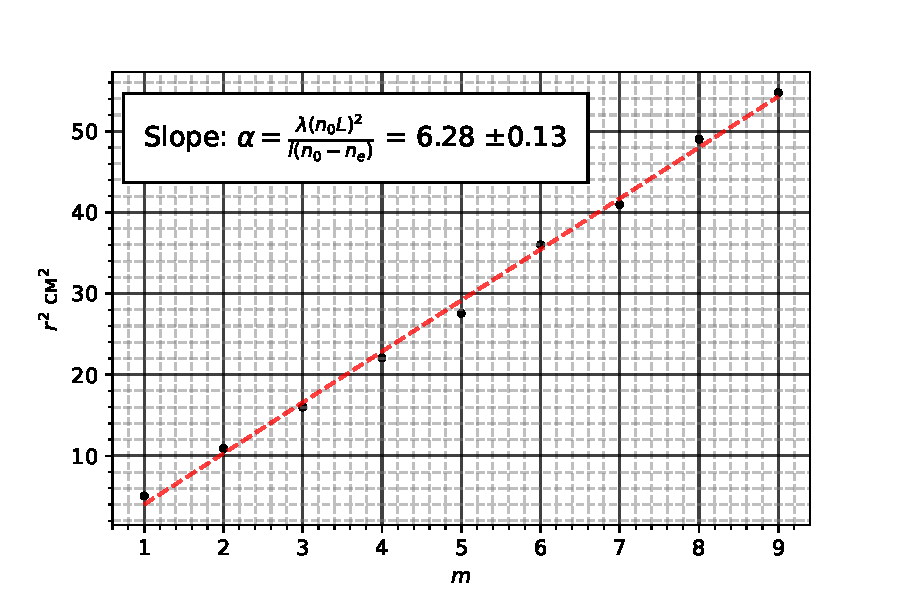
\includegraphics[scale=1]{r(m).pdf}
	\caption{График зависимости $r^2(m)$}
\end{figure}

Воспользовавшись формулой $$r_m = \frac{\lambda (n_0 L)^2}{l (n_0 - n_e)} m $$ по наклону прямой определим величину $$(n_0 - n_e)$$ таким образом получаем, что наклон прямой $$\alpha = \frac{\lambda (n_0 L)^2}{l (n_0 - n_e)} = 6.28 ~ \pm 0.13$$ $$(n_0 - n_e) = \frac{\lambda (n_0 L)^2}{l \alpha} = 0.1078$$.

Поместим кристалл в постоянное электрическое поле и определим величины $U_{\lambda/2}$ и $U_{\lambda} = 2 U_{\lambda/2}$.

\begin{center}
	$U_{\lambda/2} = 0.33$ кВ \\
	$U_{\lambda} = 0.69$ кВ \\
\end{center}

Поместим кристалл в переменное электрическое поле, выходной пучок лазера направим на фотодиод и получим на осцилографе фигуры Лиссажу.

\begin{figure}
	\centering
	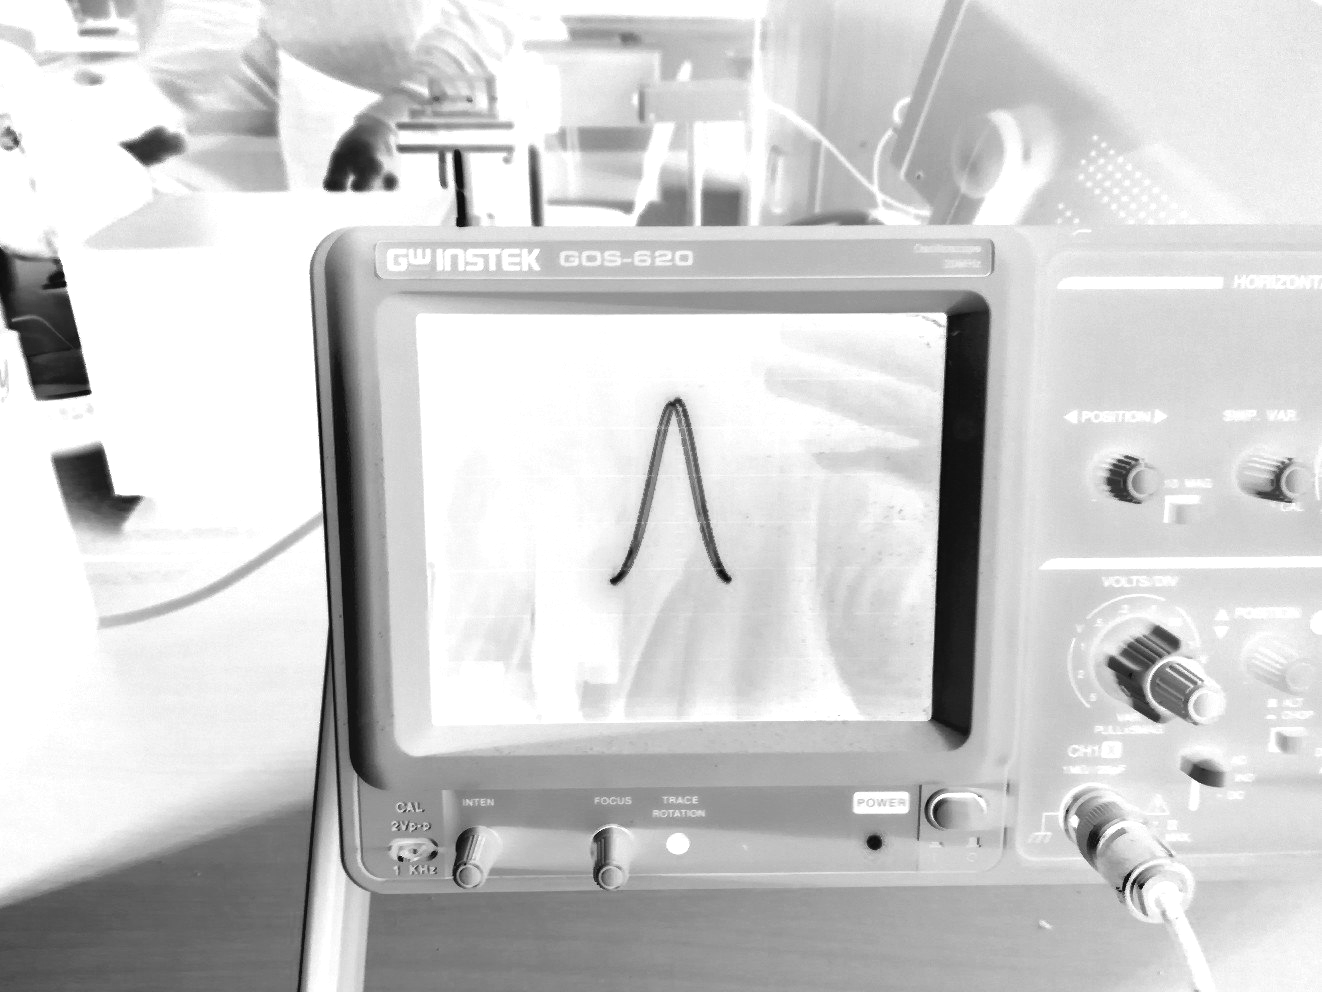
\includegraphics[scale = 0.15]{U1.png}
	\caption{Фигура Лиссажу для параллельной поляризации при амплитуде переменного напряжения $U_{\lambda/2}$}
\end{figure}

\begin{figure}
	\centering
	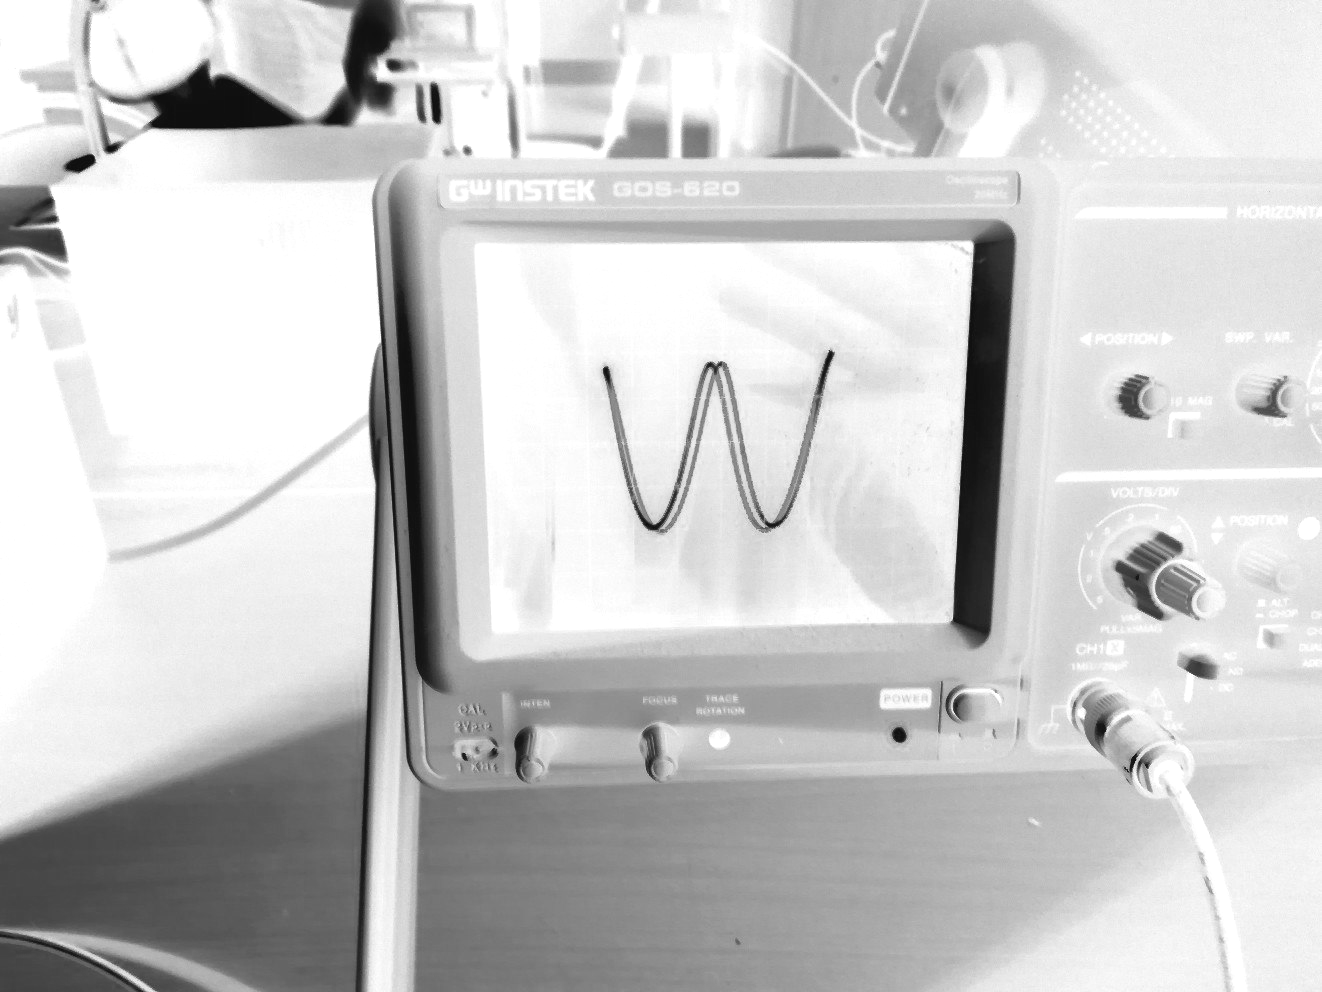
\includegraphics[scale = 0.15]{U2.png}
	\caption{Фигура Лиссажу для параллельной поляризации при амплитуде переменного напряжения $U_{\lambda}$}
\end{figure}

\begin{figure}
	\centering
	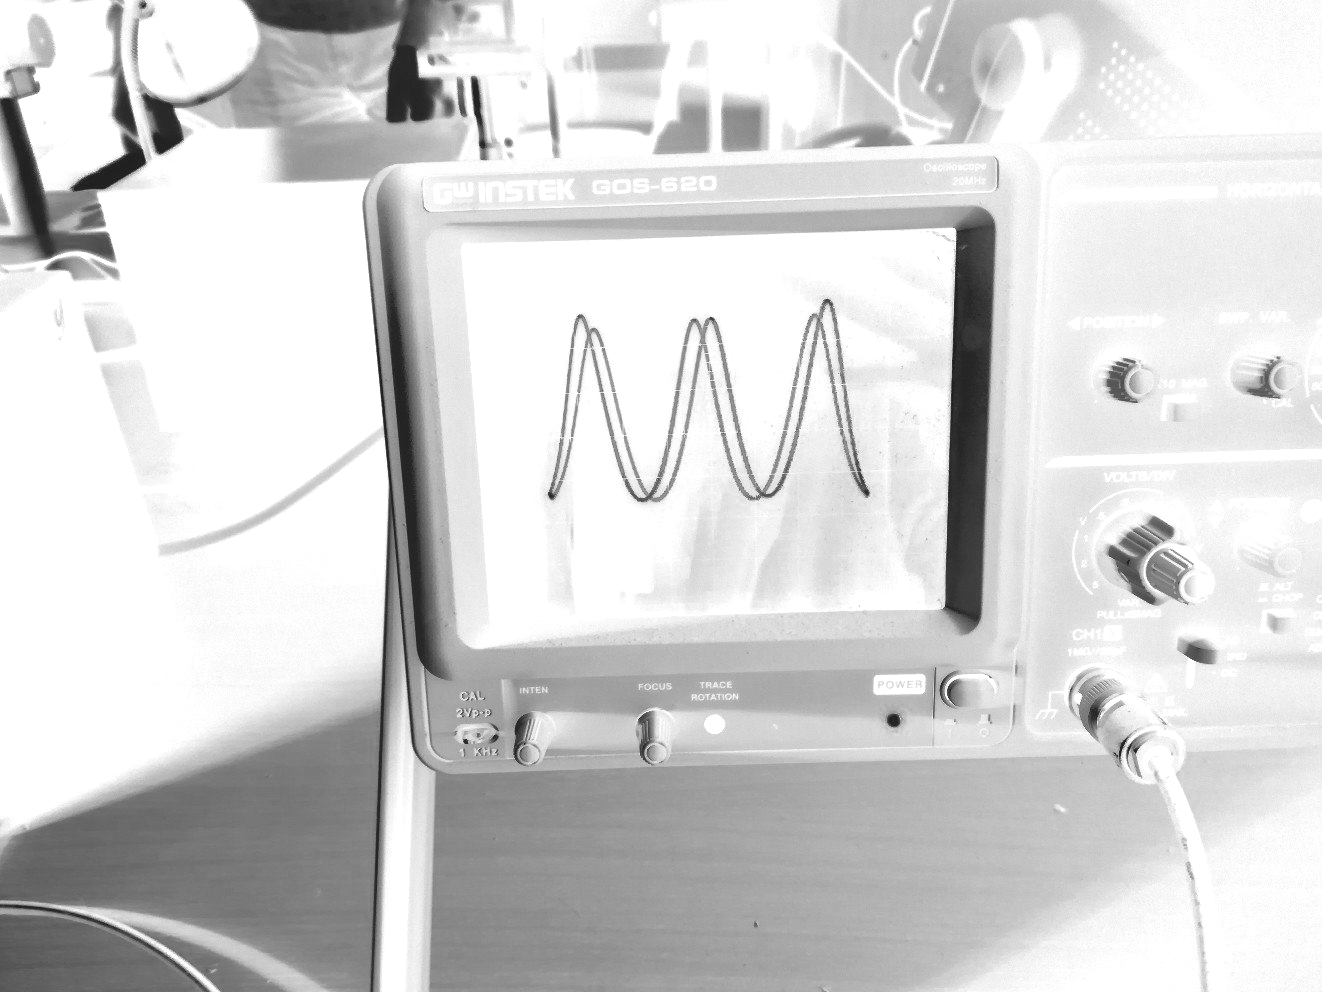
\includegraphics[scale = 0.15]{U3.png}
	\caption{Фигура Лиссажу для параллельной поляризации при амплитуде переменного напряжения $U_{3\lambda/2}$}
\end{figure} 

\end{document}